%%%%%%%%%%%%%%%%%%%%%%%%%%%%%%%%%%%%%%%%%%%%%%%%%%%%%%%%%%%%%%%%%%%%%%%%%%%%%%%%%%%%%%%%%%%%%%%%%%%%%%%%%%%%%%%%%%%%%%%% 

%%%%%%%%%%%%%%%%%%%%%%%%%%%%%%%%%%%%%%%%%%%%%%%%%%%%%%%%%%%%%%%%%%%%%%%%%%%%%%%%%%%%%%%%%%%%%%%%%%%%%%%%%%%%%%%%%%%%%%%%

%\documentclass[compress,handout]{beamer}
\documentclass[11pt,aspectratio=169,compress,mathserif]{beamer}

% lenovo native resolution is 1600x900 px, 16/9 -> 160mm by 90mm
% 1280x1024 px 5/4.

%%%%%%%%%%%%%%%%%%%%%%%%%%%%%%%%%%%%%%%%%%%%%%%%%%%%%%%%%%%%%%%%%%%%%%%%%%%%%%%%%%%%%%%%%%%%%%%%%%%%%%%%%%%%%%%%%%%%%%%%
%
% Packages
%
%%%%%%%%%%%%%%%%%%%%%%%%%%%%%%%%%%%%%%%%%%%%%%%%%%%%%%%%%%%%%%%%%%%%%%%%%%%%%%%%%%%%%%%%%%%%%%%%%%%%%%%%%%%%%%%%%%%%%%%%

\usepackage{iftex}

%**** Encoding and Font **************************

\ifPDFTeX
  \usepackage[utf8]{inputenc}
  \usepackage[T1]{fontenc}
  \usepackage{lmodern} % Postscript layout of CM with T1 coding
\else
  \ifLuaTeX
    % \usepackage[utf8]{luainputenc}
    \usepackage[T1]{fontenc}
    \usepackage{lmodern} % Postscript layout of CM with T1 coding
    %
    \hypersetup{pdfencoding=auto}
    %
    % \usepackage{fontspec} % spoil circle to square and textasteriskcentered
    % \usefontheme{professionalfonts}
    % \usepackage{unicode-math}
    % \setmathfont{Latin Modern Math}
    % \usepackage{fontawesome}
  \fi
\fi

%**** Language ***********************************

\usepackage[frenchb]{babel}
%\usepackage[english]{babel}
% \usepackage{frenchle} % compatibility?

%** Beamer ***************************************

\usepackage{beamerthemefabrice}

\usepackage{pgfpages}
%\pgfpagelayout{resize}[a4paper,border shrink=5mm,landscape]

%**** Tikz ***************************************

\usepackage{tikz}
\usetikzlibrary{calc,shapes,backgrounds,arrows}

\usepackage{graphics}

%**** Textpos ************************************

\usepackage[absolute,overlay]{textpos}
%\TPshowboxestrue
\TPshowboxesfalse
\TPGrid{16}{9}
% \textblockorigin{10mm}{10mm}

%**** Tabular ************************************

\usepackage{array}
%% \usepackage{color}
\usepackage{colortbl}
%% \usepackage{multirow}
%% \usepackage{dcolumn}
%% 
%% \usepackage{cellspace}
%% \setlength{\cellspacebottomlimit}{1pt} 
%% \setlength{\cellspacetoplimit}{1pt} 


%**** Color **************************************

\usepackage{xcolor}

%**** Units and number ***************************

% \usepackage{unite}

%*************************************************

%\usepackage{alltt}
\usepackage{fancyvrb}
\usepackage[framemethod=TikZ]{mdframed}

%%%%%%%%%%%%%%%%%%%%%%%%%%%%%%%%%%%%%%%%%%%%%%%%%%%%%%%%%%%%%%%%%%%%%%%%%%%%%%%%%%%%%%%%%%%%%%%%%%%%%%%%%%%%%%%%%%%%%%%%
%%%
%%% Local Variables: 
%%% mode: latex
%%% TeX-master: "master"
%%% End: 
%%%
%%%%%%%%%%%%%%%%%%%%%%%%%%%%%%%%%%%%%%%%%%%%%%%%%%%%%%%%%%%%%%%%%%%%%%%%%%%%%%%%%%%%%%%%%%%%%%%%%%%%%%%%%%%%%%%%%%%%%%%%

%%%%%%%%%%%%%%%%%%%%%%%%%%%%%%%%%%%%%%%%%%%%%%%%%%%%%%%%%%%%%%%%%%%%%%%%%%%%%%%%%%%%%%%%%%%%%%%%%%%%%%%%%%%%%%%%%%%%%%%%
%
% Settings
%
%%%%%%%%%%%%%%%%%%%%%%%%%%%%%%%%%%%%%%%%%%%%%%%%%%%%%%%%%%%%%%%%%%%%%%%%%%%%%%%%%%%%%%%%%%%%%%%%%%%%%%%%%%%%%%%%%%%%%%%%

% Beamer %%%%%%%%%%%%%%%%%%%%%%%%%%%%%%%%%%%%%%%%%%%%%%%%%%%%%%%%%%%%%%%%%%%%%%%%%%%%%%%%%%%%%%%%%%%%%%%%%%%%%%%%%%%%%%%

\mode<presentation>
{
  \usetheme{fabrice}
  % \usetheme{Madrid}
  % \usetheme{Warsaw}

  \setbeamersize{text margin left=5mm}
  \setbeamersize{text margin right=5mm}

  \setbeamertemplate{navigation symbols}{}
  % \setbeamertemplate{blocks}[rounded][shadow=false] % done
  \setbeamertemplate{itemize items}[circle]
  \setbeamertemplate{enumerate items}[circle]

  % \setbeamercovered{transparent}

  % \setbeamertemplate{background}[grid][step=10mm]
}

\setbeameroption{hide notes}
% \setbeameroption{show notes}
% \setbeameroption{show notes on second screen}
% \setbeameroption{show only notes}

% Comment this, if you do not want the table of contents to pop up at the beginning of each subsection:
% \AtBeginSubsection[]
% {
%  \begin{frame}<beamer>
%    \frametitle{Outline}
%    \tableofcontents[currentsection,currentsubsection]
%  \end{frame}
% }

% If you wish to uncover everything in a step-wise fashion, uncomment the following command: 
% \beamerdefaultoverlayspecification{<+->}

%%%%%%%%%%%%%%%%%%%%%%%%%%%%%%%%%%%%%%%%%%%%%%%%%%%%%%%%%%%%%%%%%%%%%%%%%%%%%%%%%%%%%%%%%%%%%%%%%%%%%%%%%%%%%%%%%%%%%%%%
%%%
%%% Local Variables: 
%%% mode: latex
%%% TeX-master: "master"
%%% End: 
%%%
%%%%%%%%%%%%%%%%%%%%%%%%%%%%%%%%%%%%%%%%%%%%%%%%%%%%%%%%%%%%%%%%%%%%%%%%%%%%%%%%%%%%%%%%%%%%%%%%%%%%%%%%%%%%%%%%%%%%%%%%

%%%%%%%%%%%%%%%%%%%%%%%%%%%%%%%%%%%%%%%%%%%%%%%%%%%%%%%%%%%%%%%%%%%%%%%%%%%%%%%%%%%%%%%%%%%%%%%%%%%%%%%%%%%%%%%%%%%%%%%%

% keep tikz
% tikzpicture ???

% Redefinition, symbol included in link:
\let\orighref\href
%\renewcommand{\href}[2]{\orighref{#1}{#2\,\resizebox{!}{1.mm}{\faExternalLink}}} % lualatex
% \pgfdeclareimage[height=1mm]{externalLink}{images/external-link-small.png}
\renewcommand{\href}[2]{%
\orighref{#1}{#2\,%
  \begin{tikzpicture}[scale=.1, mystyle/.style={line width=.25pt, line cap=round, rounded corners=.5pt}]
    \draw[mystyle] (1,.4) -- (1,0) -- (0,0) -- (0,1) -- (.7,1);
    \fill (.8,1.2) -- ++(.5,0) -- ++(0,-.5);
    \draw[mystyle] (.6,.4) -- (1.1,1.);
  \end{tikzpicture}%
%\pgfuseimage{externalLink}
}}

%%%%%%%%%%%%%%%%%%%%%%%%%%%%%%%%%%%%%%%%%%%%%%%%%%%%%%%%%%%%%%%%%%%%%%%%%%%%%%%%%%%%%%%%%%%%%%%%%%%%%%%%%%%%%%%%%%%%%%%%

\newcommand{\ptr}{\textasteriskcentered}
\newcommand{\code}[1]{\texttt{#1}}

%%%%%%%%%%%%%%%%%%%%%%%%%%%%%%%%%%%%%%%%%%%%%%%%%%%%%%%%%%%%%%%%%%%%%%%%%%%%%%%%%%%%%%%%%%%%%%%%%%%%%%%%%%%%%%%%%%%%%%%%

\newcommand{\colorR}[1]{{\color{red!80!black}#1}}
\newcommand{\colorG}[1]{{\color{green!80!black}#1}}
\newcommand{\colorB}[1]{{\color{blue!80!black}#1}}
\newcommand{\bgR}{red!20!white}

\newcommand{\boxR}[1]{\colorbox{red!20!white}{#1}}
\newcommand{\boxG}[1]{\colorbox{green!20!white}{#1}}
\newcommand{\boxB}[1]{\colorbox{blue!20!white}{#1}}

%%%%%%%%%%%%%%%%%%%%%%%%%%%%%%%%%%%%%%%%%%%%%%%%%%%%%%%%%%%%%%%%%%%%%%%%%%%%%%%%%%%%%%%%%%%%%%%%%%%%%%%%%%%%%%%%%%%%%%%%

\pgfdeclareimage[height=2cm]{FunnyPython}{images/funny-python.png}
\pgfdeclareimage[height=10mm]{FunnyPythonSmall}{images/funny-python.png}
\pgfdeclareimage[height=1cm]{OpenGLLogo}{images/khronos-logos/OpenGL/OpenGL_500.jpg}

%%%%%%%%%%%%%%%%%%%%%%%%%%%%%%%%%%%%%%%%%%%%%%%%%%%%%%%%%%%%%%%%%%%%%%%%%%%%%%%%%%%%%%%%%%%%%%%%%%%%%%%%%%%%%%%%%%%%%%%%

% raise !
\newcommand{\attention}{%
  \begin{tikzpicture}
    \node [fill=yellow!80, isosceles triangle, shape border rotate=90, inner sep=.1pt, rounded corners=1.5pt] {\textbf{!}};
  \end{tikzpicture}}

% check beamer code
\newcommand{\numberItem}[1]{
  \begin{tikzpicture}
    \node[circle, fill=blue!70!black, draw=none, inner sep = .5pt] at (0,0)
    {\textcolor{white}{\scriptsize #1}};
  \end{tikzpicture}}

%%%%%%%%%%%%%%%%%%%%%%%%%%%%%%%%%%%%%%%%%%%%%%%%%%%%%%%%%%%%%%%%%%%%%%%%%%%%%%%%%%%%%%%%%%%%%%%%%%%%%%%%%%%%%%%%%%%%%%%%
%%%
%%% Local Variables: 
%%% mode: latex
%%% TeX-master: "master"
%%% End: 
%%%
%%%%%%%%%%%%%%%%%%%%%%%%%%%%%%%%%%%%%%%%%%%%%%%%%%%%%%%%%%%%%%%%%%%%%%%%%%%%%%%%%%%%%%%%%%%%%%%%%%%%%%%%%%%%%%%%%%%%%%%%


%%%%%%%%%%%%%%%%%%%%%%%%%%%%%%%%%%%%%%%%%%%%%%%%%%%%%%%%%%%%%%%%%%%%%%%%%%%%%%%%%%%%%%%%%%%%%%%%%%%%%%%%%%%%%%%%%%%%%%%%

\title[]{Circuit Simulation using Python}
\author[F.~Salvaire]{Fabrice~Salvaire}
% \institute{} % hack since author is used in the PDF metadata
\date[13 June 17]{PyParis 2017}

\pgfdeclareimage[interpolate=true,height=3cm]{ControlledSource}{figures/controlled-source.pdf}
\logo{\pgfuseimage{FunnyPython}}
\titlegraphic{\pgfuseimage{ControlledSource}}

%%%%%%%%%%%%%%%%%%%%%%%%%%%%%%%%%%%%%%%%%%%%%%%%%%%%%%%%%%%%%%%%%%%%%%%%%%%%%%%%%%%%%%%%%%%%%%%%%%%%%%%%%%%%%%%%%%%%%%%%

\begin{document}

%%%%%%%%%%%%%%%%%%%%%%%%%%%%%%%%%%%%%%%%%%%%%%%%%%%%%%%%%%%%%%%%%%%%%%%%%%%%%%%%%%%%%%%%%%%%%%%%%%%%%%%%%%%%%%%%%%%%%%%%
%
%                                                       Title Page
%
%%%%%%%%%%%%%%%%%%%%%%%%%%%%%%%%%%%%%%%%%%%%%%%%%%%%%%%%%%%%%%%%%%%%%%%%%%%%%%%%%%%%%%%%%%%%%%%%%%%%%%%%%%%%%%%%%%%%%%%%

\begin{frame} % Title Page Frame
  \titlepage
  \begin{textblock}{12}(.2,7)
    % \tiny%
    \fontsize{5pt}{5pt}\selectfont
    \url{http://pyparis.org} \\[.5em]
    \texttt{\url{https://www.fabrice-salvaire.fr/en/about/contact}} \\ % contact fabrice.salvaire.fr
    \url{https://github.com/FabriceSalvaire/pyparis-2017} \\[.5em]
    CC BY-NC-SA 3.0 \\[2em]
    \fontsize{7pt}{7pt}\selectfont
    \url{https://pyspice.fabrice-salvaire.fr/pyparis-2017-talk.pdf}
\end{textblock}
\end{frame}

\logo{} % hack to clear the logo

%%%%%%%%%%%%%%%%%%%%%%%%%%%%%%%%%%%%%%%%%%%%%%%%%%%%%%%%%%%%%%%%%%%%%%%%%%%%%%%%%%%%%%%%%%%%%%%%%%%%%%%%%%%%%%%%%%%%%%%%
%
%                                                       Outline
%
%%%%%%%%%%%%%%%%%%%%%%%%%%%%%%%%%%%%%%%%%%%%%%%%%%%%%%%%%%%%%%%%%%%%%%%%%%%%%%%%%%%%%%%%%%%%%%%%%%%%%%%%%%%%%%%%%%%%%%%%

% pour l'impression recto-verso
% \frame{}

\frame{%
\tableofcontents
\note{
}
}

%%%%%%%%%%%%%%%%%%%%%%%%%%%%%%%%%%%%%%%%%%%%%%%%%%%%%%%%%%%%%%%%%%%%%%%%%%%%%%%%%%%%%%%%%%%%%%%%%%%%%%%%%%%%%%%%%%%%%%%%
%
%                                             Sections
%
%%%%%%%%%%%%%%%%%%%%%%%%%%%%%%%%%%%%%%%%%%%%%%%%%%%%%%%%%%%%%%%%%%%%%%%%%%%%%%%%%%%%%%%%%%%%%%%%%%%%%%%%%%%%%%%%%%%%%%%%

% ???
% 
\begin{frame}
  \frametitle{Author Bio}
  In few words
  \begin{itemize}
  \item \href{https://www-h1.desy.de/psfiles/ps4/theses/h1th-464.pdf}{PhD} in High Energy Physics at \href{http://www.desy.de}{DESY}
  \item Worked as project manager in the industry
  \item Participated to the construction of the largest European hackerspace \href{http://www.electrolab.fr}{Electrolab}
  \end{itemize}
\end{frame}

%%% Local Variables:
%%% mode: latex
%%% TeX-master: "master"
%%% End:


\section{Why Python is the right language for engineering ?}

\section{An Introduction to Circuit Simulation}

\begin{frame}
  \frametitle{Circuit Simulation: Nodal Analysis}
  \begin{columns}
    \begin{column}{.5\textwidth}
      \begin{center}
        \textbf{Circuit $\equiv$ Device's Graph} \\[1em]
        \includegraphics[width=1.\textwidth]{figures/network.pdf}
      \end{center}
    \end{column}
    \begin{column}{.5\textwidth}
      \textit{Roughly \ldots} \\[1em]
      \begin{enumerate}
      \item Apply \textbf{Kirchhoff's} circuit laws
        \begin{itemize}
        \item Kirchhoff's current law (KCL) \\
          $\sum {I}_k = 0$ for each node \\
          \textit{conservation of the electron flow} \\[.5em]
        \item Kirchhoff's voltage law (KVL) \\
          $\sum {V}_k = 0$ for each cycle \\
          \textit{think that is a closed path} \\[1em]
        \end{itemize}
      \item Apply \textbf{Device Equation} $f(V_k,I_k) = 0$ \\
        e.g.\@ Ohm Law for resistor $V = R I$ \\[.5em]
        Can be \textbf{Complex} e.g.\@ Capacitor, Inductor \\
        and \textbf{Non-Linear} e.g. Diode !
      \end{enumerate}
    \end{column}
  \end{columns}
\end{frame}

\begin{frame}
  \frametitle{Circuit Simulation: Nodal Analysis Example}
  \begin{columns}
    \begin{column}{.3\textwidth}
      \begin{center}
        \includegraphics[width=1.\textwidth]{figures/nodal-analysis.pdf}
      \end{center}
    \end{column}
    \begin{column}{.7\textwidth}
      Let apply the recipes: % Kirchhoff's circuit laws
      $$
      \begin{pmatrix}
        \frac{1}{R_1}+\frac{1}{R_2} & -\frac{1}{R_2} & 1 \\
        -\frac{1}{R_2} & \frac{1}{R_2}+\frac{1}{R_3} & -1 \\
        1 & -1 & 0
      \end{pmatrix}
      { \color{red!80}
      \begin{bmatrix}
        V_1 \\
        V_2 \\
        I_{V_{s1}}
      \end{bmatrix}
      }
      =
      \begin{bmatrix}
        I_{s1} \\
        0 \\
        V_{s1}
      \end{bmatrix}
      $$
      Then \textbf{solve} this \textbf{system of linear equations} \\[1em]
      There are \textbf{algorithms} to build theses \textbf{matrices} \\
      Usually matrices are \textbf{sparses} \\[1em]
      \textbf{Complex} therms for Capacitor, Inductor e.g.\@ $V^\star = \frac{1}{sC} I^\star$ % $V^\star = sL I^\star$
      \\[.5em]
      \textbf{Non linear} e.g.\@ Shockley Diode Model $I = I_s \left( e^{\frac{V}{n V_T}} - 1 \right)$
      \\[1em]
      {\tiny
        To go further \href{http://qucs.sourceforge.net/tech/technical.html}{QUCS Technical Papers}
        or \href{http://qucs.sourceforge.net/docs/technical/technical.pdf}{PDF}
      }
    \end{column}
  \end{columns}
\end{frame}


\begin{frame}
  \frametitle{Circuit Simulation: Several kinds of Analysis}
  \begin{columns}
    \begin{column}[t]{.6\textwidth}
      Principal Analyses \\[1em]
      \begin{itemize}
      \item DC Analysis \\
        \textit{Operating Point and DC Sweep} \\
        Compute node's voltages at $t=0$
        \textbf{cf. infra} \\[1em]
      \item AC Small-Signal Analysis \\
        \textbf{Transfer Function} \\
        Frequency Analysis $V(\omega)$, cf. Laplace Transform \\
        \textit{small means Taylor Series} \\[1em]
      \item Transient Analysis \\
        Simulate over time $V(t)$ \\
        \textbf{Integrator}
      \end{itemize}
    \end{column}
    \begin{column}[t]{.4\textwidth}
      More specific ones \\[1em]
      \begin{itemize}
      \item Pole-Zero Analysis
      \item Small-Signal Distortion Analysis
      \item Sensitivity Analysis
      \item Noise Analysis
      \item etc.\@
      \end{itemize}
    \end{column}
  \end{columns}
\end{frame}

%%% Local Variables:
%%% mode: latex
%%% TeX-master: "master"
%%% End:


\section{SPICE an Industrial Standard}

\begin{frame}
  \frametitle{SPICE: Simulation Program with Integrated Circuit Emphasis}
  \begin{columns}
    \begin{column}{.7\textwidth}
      % In few words
      \begin{itemize}
      \item Developed by Dr. Laurence Nagel in 1973 at Berkeley % University of California
      \item \textbf{First software} to combine \\
        DC, AC and transient analog circuit analysis capabilities
      \item An early \textbf{open source} software initiative (Public Domain)
      \item \textbf{Used in undergraduate courses}
      \item \textbf{Evolved to a worldwide standard} % integrated circuit simulator
      \item \textbf{IEEE Milestone} on February 4, 2011
      \item Berkeley released spice3f5 on 1993 % 6
      \item Superseded by commercial and open source forks
      \end{itemize}
      % What it does ?
      % \begin{itemize}
      % \item Netlist language to describe circuit
      % \item Simulator
      % \end{itemize}
      {\tiny To go further
        \href{https://www2.eecs.berkeley.edu/Pubs/TechRpts/1975/9602.html}%
        {SPICE2: A Computer Program to Simulate Semiconductor Circuits; Nagel, Laurence W.; 1975}
      }
    \end{column}
    \begin{column}{.3\textwidth}
      \begin{center}
        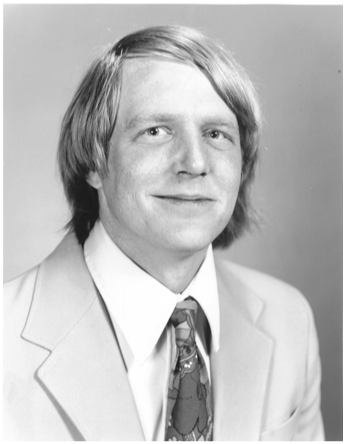
\includegraphics[height=3cm]{images/Larry-Nagel-portrait-young.png} \\[1cm]
        
\includegraphics[width=.7\textwidth]{images/Nagel_Plaque-SCV-2016.png}
      \end{center}
    \end{column}
  \end{columns}
\end{frame}

\begin{frame}[fragile]
  \frametitle{SPICE: Netlist}
  \begin{columns}
    \begin{column}{.5\textwidth}
      \begin{center}
        \includegraphics[width=.9\textwidth]{figures/ac-coupled-amplifier.pdf}
      \end{center}
    \end{column}
    \begin{column}{.5\textwidth}
     {\footnotesize
\begin{verbatim}
AC-coupled amplifier
Vpwr 6 0 DC 15V
Vin 1 0 AC 1V SIN(0V .5V 1KHz)
C1 1 2 10u
R1 6 2 100k
R2 2 0 20k
RC 6 4 10k
Q1 4 2 3 bjt
RE 3 0 2k
C2 4 5 10u
RL 5 0 1Meg
.model bjt npn(bf=80 cjc=5p rb=100)
.ac dec 5 10m 1G
*.tran .02ms 2ms 0 .01ms
.control
run
plot V(1) V(5)
.end
\end{verbatim}%
     }
   \end{column}
 \end{columns}
\end{frame}

\begin{frame}[fragile]
  \frametitle{SPICE: A Worldwide Standard for integrated circuit simulation}
  \centerline{Device manufacturers use SPICE language to provide models as sub-circuit}
  \begin{columns}
    \begin{column}{.5\textwidth}
      \begin{center}
        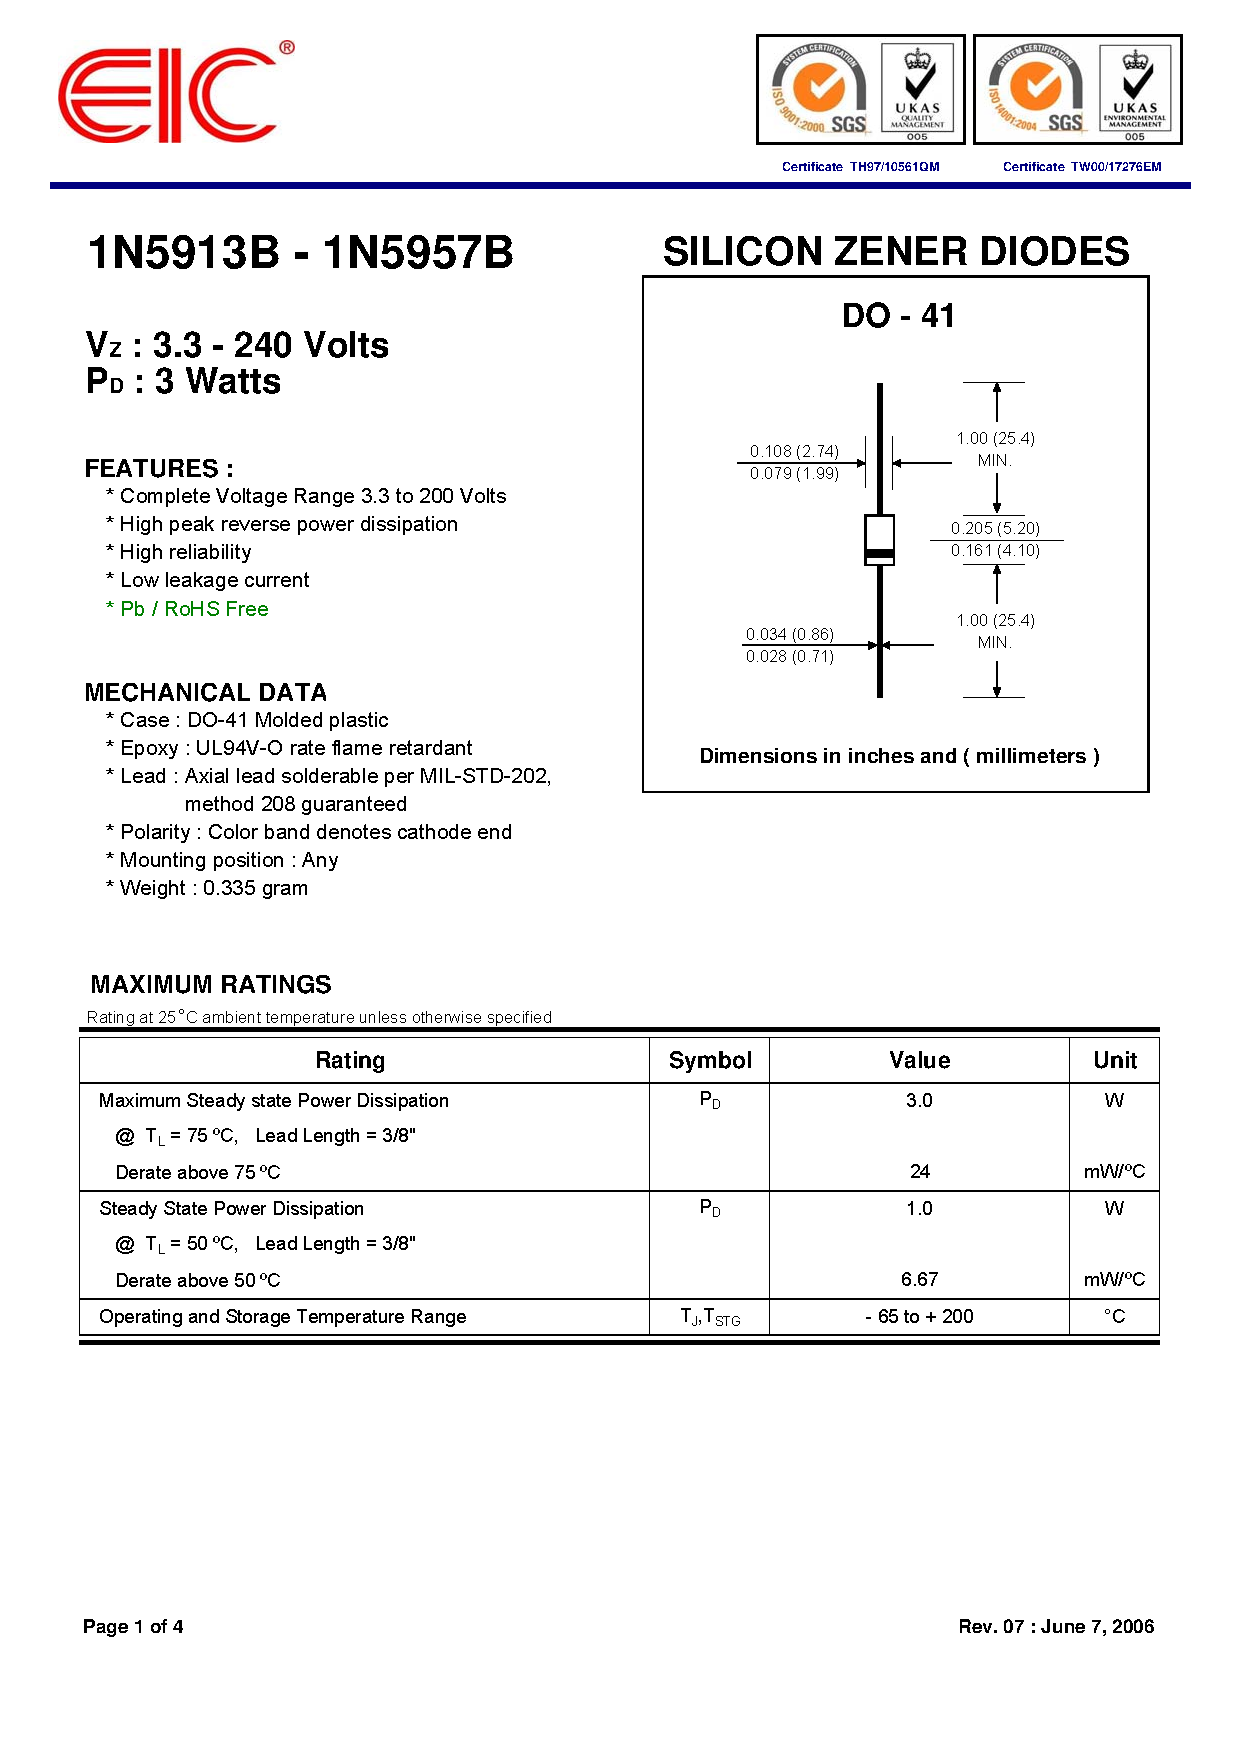
\includegraphics[height=6cm]{figures/1N5919B-1.pdf}
      \end{center}
    \end{column}
    \begin{column}{.5\textwidth}
      {\fontsize{4.25pt}{4.25pt}\selectfont
\begin{verbatim}
* http://www.onsemi.com/pub_link/Collateral/1N5919BRL.SP3
.SUBCKT d1n5919brl 2 1
**************************************
*      Model Generated by MODPEX     *
*Copyright(c) Symmetry Design Systems*
*         All Rights Reserved        *
*    UNPUBLISHED LICENSED SOFTWARE   *
*   Contains Proprietary Information *
*      Which is The Property of      *
*     SYMMETRY OR ITS LICENSORS      *
*    Modeling services provided by   *
* Interface Technologies www.i-t.com *
**************************************
* Model generated on Jun 22, 2004
* MODEL FORMAT: SPICE3
*     anode cathode
*node: 2      1
*    Forward Section
D1 2 1 MD1
.MODEL MD1 D IS=1.33275e-21 N=1 XTI=1 RS=0.1
+ CJO=1e-11 TT=1e-08
*    Leakage Current
R 1 2 600000 MDR
.MODEL MDR R TC1=0 TC2=0
*    Breakdown
RZ 2 3 0.520393
IZG 4 3 0.3204
R4 4 3 100
D3 3 4 MD3
.MODEL MD3 D IS=2.5e-12 N=2.40102 XTI=0 EG=0.1
D2 5 4 MD2
.MODEL MD2 D IS=2.5e-12 N=3.19856 XTI=0 EG=0.1
EV1 1 5 6 0 1
IBV 0 6 0.001
RBV 6 0 5153.19 MDRBV
.MODEL MDRBV R TC1=1.79e-08
*-- SPICE3 DIODE MODEL DEFAULT PARAMETER
*  VALUES ARE ASSUMED
*IS=1E-14 RS=0 N=1 TT=0 CJO=0
*VJ=1 M=0.5 EG=1.11 XTI=3 FC=0.5
*KF=0 AF=1 BV=inf IBV=1e-3 TNOM=27
.ENDS d1n5919brl
\end{verbatim}%
      }
    \end{column}
  \end{columns}
\end{frame}

%%% Local Variables:
%%% mode: latex
%%% TeX-master: "master"
%%% End:


\begin{frame}
  \frametitle{SPICE Open Source Clones: Many initiatives \ldots !}
  \begin{enumerate}
  \item \textbf{Berkeley spice3f5} \alert{1993} % 6
    \begin{itemize}
    \item A Research Project
    \item Source code \alert{was not developed with industrial Q\&A}
    \end{itemize}
  \item \textbf{Ngspice} (New Generation Spice)
    \begin{itemize}
    \item \alert{Fork of Berkeley spice3f5}
    \item Features mixed-level and mixed-signal simulation \\
      XSpice (mixed signal), Cider1b1 and GENIUS TCAD (mixed level)
    \item \alert{Still maintained (?) but not actively !}
      % \item Manual has 600 pages
    \end{itemize}
  \item \textbf{GnuCap} (GNU Circuit Analysis Package)
    \begin{itemize}
    \item Attempt to rewrite SPICE from scratch by Albert Davis in \alert{1993}
    \item Davis's Thesis "Implicit Mixed-Mode Simulation of VLSI Circuits"
    \item No longer maintained since 2006 (2013 ?)
    \end{itemize}
  \item \textbf{QUCS} (Quite Universal Circuit Simulator) \alert{2003}
  \item \textbf{Akhab} \alert{2006}
  \end{enumerate}
\end{frame}

\begin{frame}
  \frametitle{QUCS: When Open Source fails !}
  \begin{columns}
    \begin{column}{.6\textwidth}
      \centerline{QUCS: Quite Universal Circuit Simulator}
      \begin{itemize}
      \item Founded by Michael Margraf in 2003 (?)
      \item \textbf{IDE} based on Qt3 \\
      \item \textbf{Complete Toolchain} \\
        Schematic Editor, Simulation and Plot
      \item \textbf{Interesting simulation features}
      \item Margraf moved later to proprietary software ???
      \item Slowly maintained \\
        port to Qt4 is ongoing since \ldots many years
      \end{itemize}
    \end{column}
    \begin{column}{.4\textwidth}
      \begin{center}
        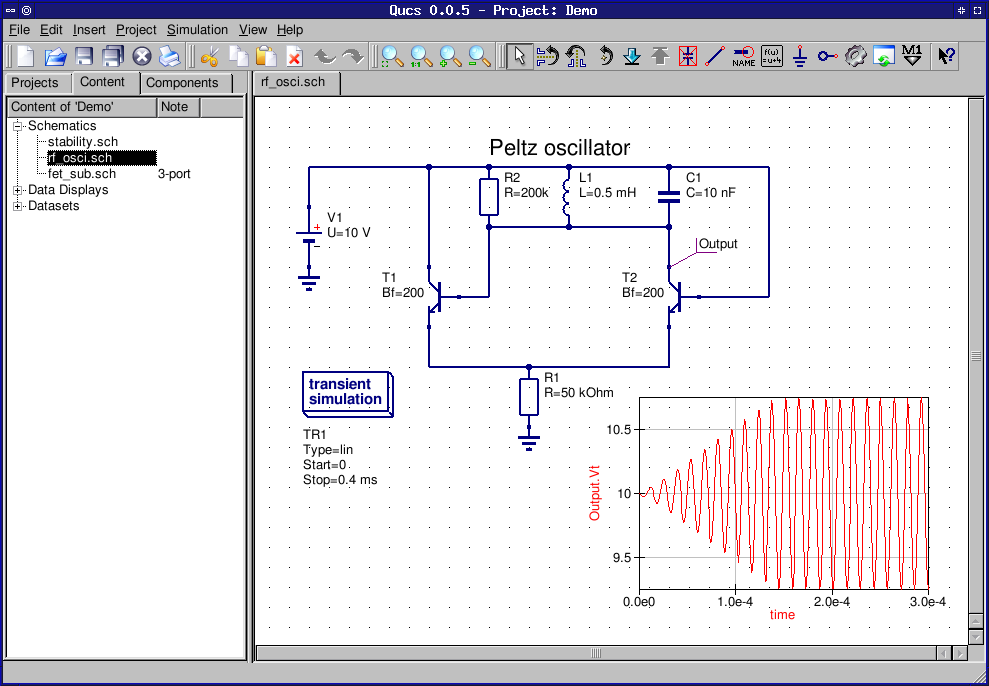
\includegraphics[width=1.\textwidth]{images/qucs.png}
      \end{center}
    \end{column}
  \end{columns}
\end{frame}

\begin{frame}
  \frametitle{QUCS: What is wrong ?}
  \begin{columns}
    \begin{column}[t]{.5\textwidth}
      To develop an electric CAD software, \\
      we need these \textbf{skills} and \textbf{budgets}
      {\footnotesize
        \begin{itemize}
        \item Circuit Simulation
        \item Solid State Device Modelling
        \item State of Art Numerical Analysis
        \item Software Architecture, Core Design
        \item GUI Design
        \item XML Format Design
        \item Schematic Editor Design
        \item Plot Library
        \item \ldots
        \end{itemize}%
      }
      \begin{textblock}{6}(4,6.5)
        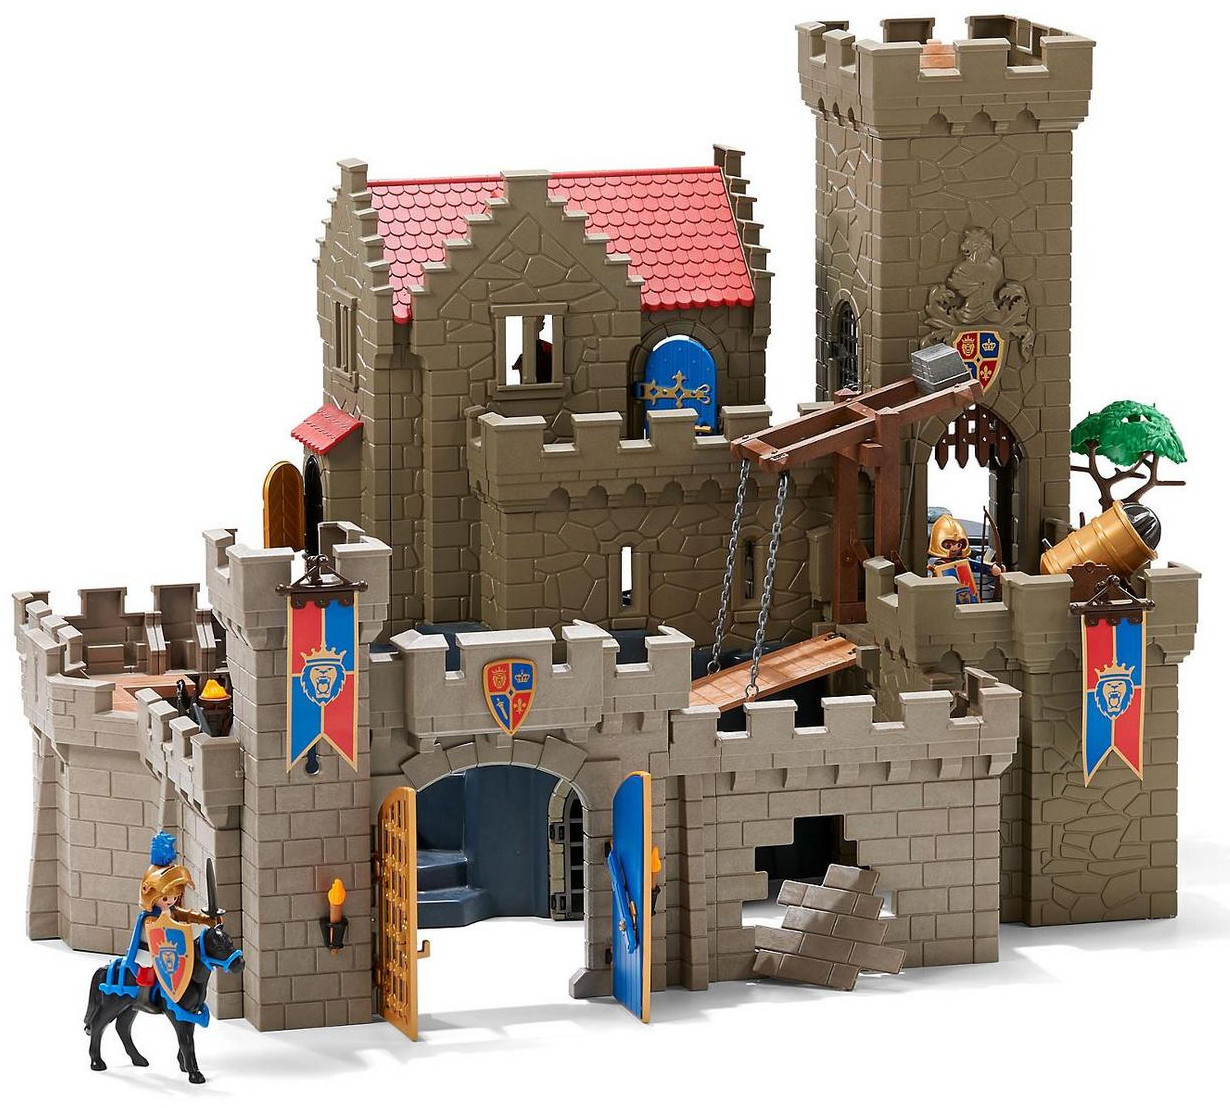
\includegraphics[width=.4\textwidth]{images/playmobil.jpg}
      \end{textblock}
    \end{column}
    \begin{column}[t]{.5\textwidth}
      Later, We have to \alert{maintain} \\[.5em]
      \begin{itemize}
        \item A very large code base
        \item A GUI Qt3 $\rightarrow$ Qt4 $\rightarrow$ Qt5 $\rightarrow$ \ldots \\[1em]
      \end{itemize}
      \alert{Don't do that} until you have a zillion \$ (industrial market) \\[1em]
      \alert{\textbf{Develop Software Components !}} \\
      \alert{\textbf{And plug them together}} \\
      
\includegraphics[width=.5\textwidth]{images/lego2.jpg}
    \end{column}
  \end{columns}
\end{frame}

%%% Local Variables:
%%% mode: latex
%%% TeX-master: "master"
%%% End:


\section{PySpice the Bridge between SPICE and Python}

\begin{frame}
  \frametitle{PySpice}
\end{frame}

\begin{frame}
  \frametitle{Akhab}
\end{frame}

%%% Local Variables:
%%% mode: latex
%%% TeX-master: "master"
%%% End:


\begin{frame}
  \frametitle{Related Project: Akhab \hspace{1em} \small{pronounced "uh, cab"}}
  \begin{itemize}
  \item \textbf{Goal} : Implement a SPICE like in Python \\
    using Numpy, SciPy, and SymPy
  \item Started by \href{http://ggventurini.io}{Giuseppe Venturini} in 2006 {\tiny $\dag$ sadly deceased at the end of 2015 $\dag$}
  \item \url{https://ahkab.github.io/ahkab} % https://ahkab.github.io/ahkab
  % \item \url{https://ahkab.readthedocs.io/en/latest}
  \item v0.18 released on July 2015
  \end{itemize}
  \begin{textblock}{4}(13,3)
    
\includegraphics[width=2cm]{images/akhab.png}
  \end{textblock}
\end{frame}

%%% Local Variables:
%%% mode: latex
%%% TeX-master: "master"
%%% End:


\section{Modelica a Language for Simulation}

\begin{frame}
  \frametitle{Modelica: A language for modelling of complex physical systems}
  % What is Modelica ?
  Modelica in few words
  \begin{itemize}
  \item A \textbf{language} and a \textbf{Standard Library}
  \item Object-Oriented and Equation based
  \item Multi-domains
  \item Non-proprietary
  \item Developed by the non-profit \textbf{Modelica Association}
  \item initiated in September 1996 by Hilding Elmqvist
  \item First version on Sept. 1997  $\rightarrow$ 3.4 on April 2017
  \item Commercial front-ends: e.g.\@ Dymola
  \item Open Source front-ends: \textbf{OpenModelica} and \textbf{JModelica} \\[1em]
  \end{itemize}
  % \begin{columns}
  %   \begin{column}[t]{.65\textwidth}
  % \end{column}
  % \begin{column}[t]{.35\textwidth}
  %   Front-Ends
  %   \begin{itemize}
  %   \item Commercial : e.g.\@ Dymola
  %   \item Open Source : \\
  %     \begin{itemize}
  %     \item OpenModelica
  %     \item JModelica
  %     \end{itemize}
  %   \end{itemize}
  % \end{column}
  % \end{columns}
  {\tiny To go further \url{https://www.modelica.org}}
  \begin{textblock}{6}(13,7)
    
\includegraphics[width=2cm]{images/modelica-logo.jpg}
  \end{textblock}
\end{frame}

\begin{frame}[fragile]
  \frametitle{Modelica: Bouncing-ball example}
  \fontsize{8pt}{8pt}\selectfont
\begin{Verbatim}[commandchars=\\\{\}]
\colorG{model} BouncingBall
  \colorG{parameter} Real e=0.7 \colorR{"coefficient of restitution"};
  \colorG{parameter} Real g=9.81 \colorR{"gravity acceleration"};
  Real h(start=1) \colorR{"height of ball"};
  Real v \colorR{"velocity of ball"};
  Boolean flying(start=true) \colorR{"true, if ball is flying"};
  Boolean impact;
  Real v_new;

\colorM{equation}
  impact = h <= 0;
  \colorB{der}(v) = \colorM{if} flying \colorM{then} -g \colorM{else} 0;
  \colorB{der}(h) = v;

  \colorO{// Triggered when one of theses conditions are true}
  \colorM{when} \{h <= 0 \colorM{and} v <= 0, impact\} \colorM{then}
    v_new = \colorM{if} \colorB{edge}(impact) \colorM{then} -e*\colorB{pre}(v) \colorM{else} 0;
    flying = v_new > 0;
    \colorB{reinit}(v, v_new);
  \colorM{end when};

\colorG{end} BouncingBall;
\end{Verbatim}
  \normalsize
\end{frame}

%%% Local Variables:
%%% mode: latex
%%% TeX-master: "master"
%%% End:


\end{document}

%%%%%%%%%%%%%%%%%%%%%%%%%%%%%%%%%%%%%%%%%%%%%%%%%%%%%%%%%%%%%%%%%%%%%%%%%%%%%%%%%%%%%%%%%%%%%%%%%%%%%%%%%%%%%%%%%%%%%%%%
%%%
%%% Local Variables: 
%%% mode: latex
%%% TeX-master: t
%%% End: 
%%%
%%%%%%%%%%%%%%%%%%%%%%%%%%%%%%%%%%%%%%%%%%%%%%%%%%%%%%%%%%%%%%%%%%%%%%%%%%%%%%%%%%%%%%%%%%%%%%%%%%%%%%%%%%%%%%%%%%%%%%%%
